\section[Optimal Control of Pitch/Travel without Feedback]{\setstretch{0.5}Optimal Control of Pitch/Travel \\ without Feedback}\label{sec:10.2}

In this section an optimal trajectory $x^*$ and a corresponding optimal input sequence $u^*$ is calculated. The calculated trajectory is used to bring the helicopter from its initial state to a desired final state. Elevation and feedback of the measured state are disregarded in this section.

\subsection{Continuous time state space form}
The model of the system can be written on continuous state space form 

\begin{equation}
\dot x = {A_c}x + {B_c}u
\end{equation}
\label{eq:statespace}

where $x=[\lambda\quad r\quad p\quad \dot p]^\top$ and $u=p_c$. The system matrices $A_c$ and $B_c$ are given by

\begin{subequations}
\begin{equation}
{A_c} = \left[ {\begin{array}{*{20}{c}}
0&1&0&0\\
0&0&{ - {K_2}}&0\\
0&0&0&1\\
0&0&{ - {K_1}{K_{pp}}}&{ - {K_1}{K_{pd}}}
\end{array}} \right]
\end{equation}\\
\begin{equation}
{B_c} = \left[ {\begin{array}{*{20}{c}}
0\\
0\\
0\\
{{K_1}{K_{pp}}}
\end{array}} \right]
\end{equation}
\end{subequations}\\

The model includes the basic control layer and the physical layer. The basic control layer consist of a PD controller for elevation control and a PID controller for pitch control, while the physical layer consist of the states connected to the helicopter. In regard to Figure \ref{fig:controlhierch}, which describes the system, the model is the two lower layers. The optimization layer is the layer we will focus on in this report. The optimal input sequence $u^*$ calculated will be implemented as setpoints for the inner controllers in the basic control layer.

\begin{figure}[H]
\includegraphics{figures/openLoopFlowChart}
\centering
\caption{Illustration of the layers in the control hierarchy}\label{fig:controlhierch}
\end{figure}

\subsection{Discrete time state space form}
The model is discretized by using the forward Euler method, given by
\begin{subequations}
\begin{equation}
{x_{k + 1}} = {x_k} + \Delta t({A_c}{x_k} + {B_c}{u_k})
\end{equation}
\begin{equation}
{x_{k + 1}} = (I + \Delta t{A_c}){x_k} + (\Delta t{B_c}){u_k}
\end{equation}
\label{eq:forwardeuler}
\end{subequations}

Thus, the model can be written on discrete time state space form
\begin{equation}
{x_{k + 1}} = A{x_k} + B{u_k}
\end{equation}

where 

\begin{subequations}
\begin{equation}
A = I + \Delta t{A_c} = \left[ {\begin{array}{*{20}{c}}
1&\Delta t&0&0\\
0&1&{ - \Delta t{K_2}}&0\\
0&0&1&\Delta t\\
0&0&{ - \Delta t{K_1}{K_{pp}}}&{1 - \Delta t{K_1}{K_{pd}}}
\end{array}} \right]
\end{equation}\\

\begin{equation}
B = \Delta t{B_c} = \left[ {\begin{array}{*{20}{c}}
0\\
0\\
0\\
{\Delta t{K_1}{K_{pp}}}
\end{array}} \right]
\end{equation}
\end{subequations}

\subsection{Optimizing problem}
An optimal trajectory for moving the helicopter from ${x_0}=[{\lambda_0}\quad 0\quad 0\quad 0]^\top$ to ${x_f}=[{\lambda_f}\quad 0\quad 0\quad 0]^\top$ is calculated. The elevation angle is assumed to be constant. ${\lambda_0}$ is set to $\pi$, and ${\lambda_f}$ is set to 0. A constraint to the pitch state is implemented, such that

\begin{equation}
|{p_k}| \le \frac{{30\pi }}{{180}},\quad k \in \{ 1, \ldots ,N\}
\end{equation}

The optimal trajectory is found by minimizing the cost function 

\begin{equation}
\phi  = \sum\limits_{i = 1}^N {{{({\lambda _i} - {\lambda _f})}^2} + qp_{ci}^2},\quad 
q \ge 0
\end{equation}

by using the built-in MATLAB function \texttt{quadprog}. The cost function is minimized with the weight parameter $q$ set to 0.1, 1 and 10. A sampling time of 0.25 s is used over a horizon of $N = 100$. 

The minimization of the cost function gives the optimal input sequence $u^*$. 20 zeros are added to the input vector to get the helicopter to stabilize after start-up, and keep it at $x_0$ for five seconds before starting to move towards its desired state. Furthermore, 30$\degree$ are subtracted from the elevation measurement to get the helicopter to fly at a reasonable height with $e_c = 0$. 

\begin{figure}[H]
\captionsetup{justification=centering}
\includegraphics[width=1\linewidth]{figures/simuling_model_1024}
\centering
\caption{Simulink model for optimal control of pitch/travel without feedback}\label{fig:simulink_10_2} 
\end{figure}

Figure \ref{fig:simulink_10_2} shows the Simulink model that is used for this part of the exercise. The figure clearly shows that no feedback is implemented for the optimal input sequence $u^*$ and optimal trajectory $x^*$, which are obtained from the MATLAB-script via the \texttt{From Workspace}-block.

\subsection{Results and discussion}
The calculated trajectories for input ($u$), travel ($\lambda$) and pitch ($p$) for $q = 0.1$, $1$, and $10$ are shown in Figure \ref{fig:10_2_q_0.1}, \ref{fig:10_2_q_1} and \ref{fig:10_2_q_10} below.

\begin{figure}[H]
    \centering
    \captionsetup{justification=centering}
    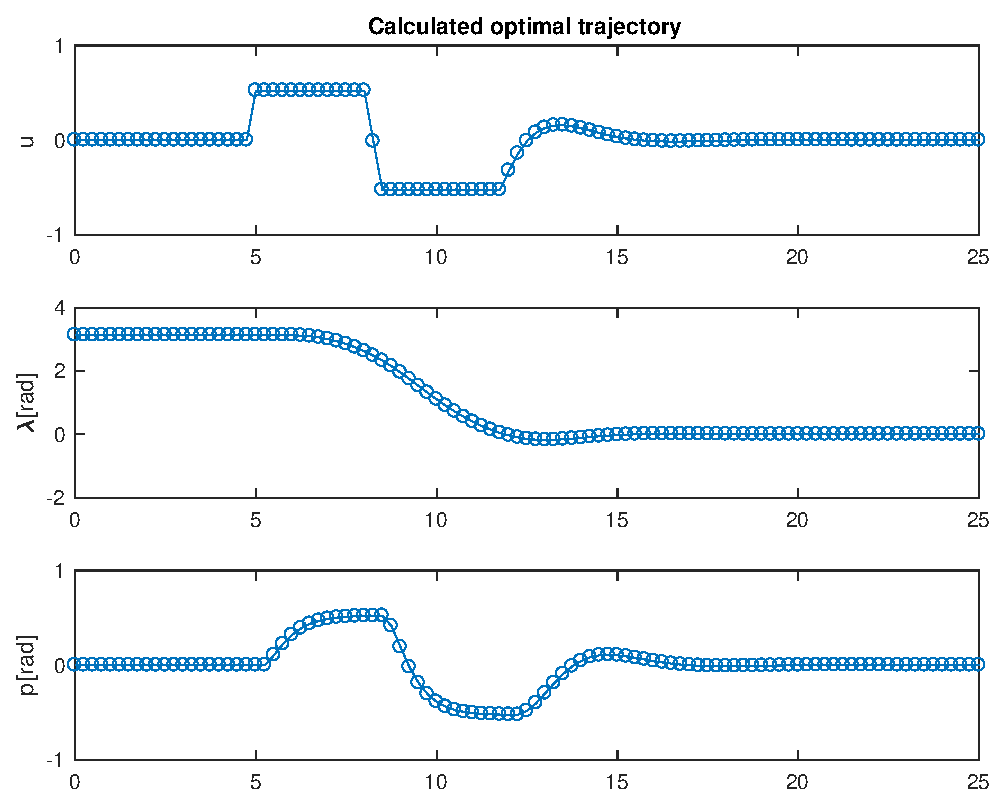
\includegraphics[scale=0.5]{data_10.2/All_states_q_1000000e-01.eps}
    \caption{Calculated optimal trajectory showing input ($u$), travel ($\lambda$) and pitch ($p$) with $q = 0.1$.}
    \label{fig:10_2_q_0.1}
\end{figure}

\begin{figure}[H]
    \centering
    \captionsetup{justification=centering}
    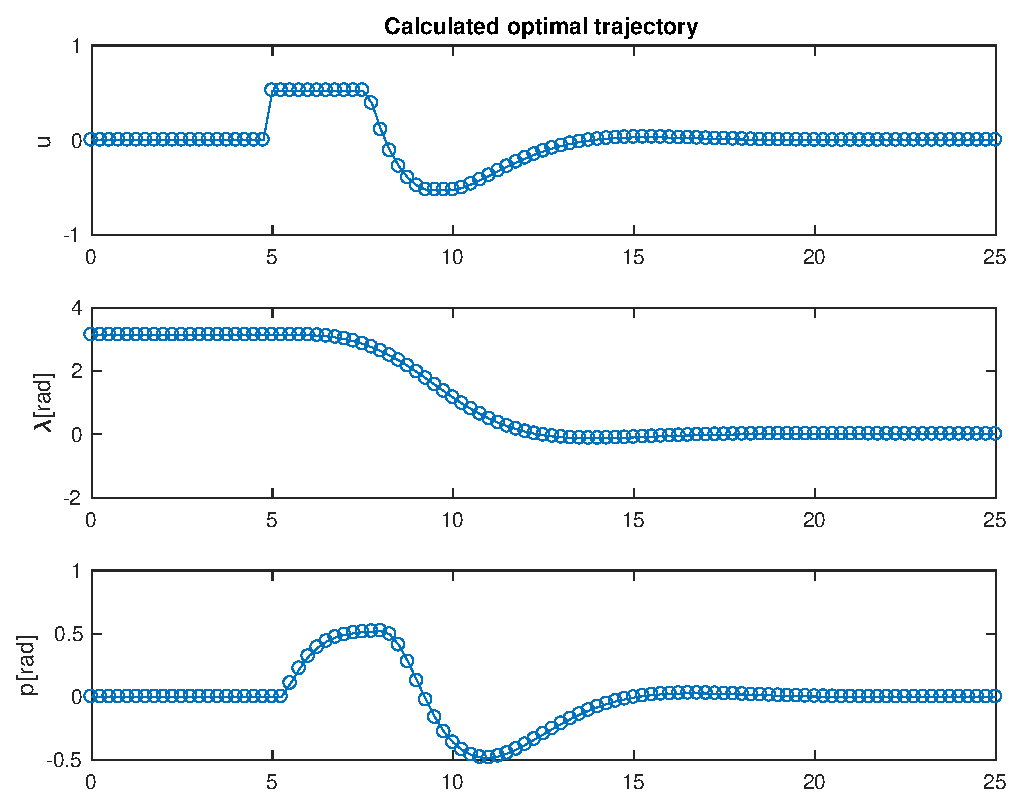
\includegraphics[scale=0.5]{data_10.2/All_states_q_1.eps}
    \caption{Calculated optimal trajectory showing input ($u$), travel ($\lambda$) and pitch ($p$) with $q = 1$.}
    \label{fig:10_2_q_1}
\end{figure}

\begin{figure}[H]
    \centering
    \captionsetup{justification=centering}
    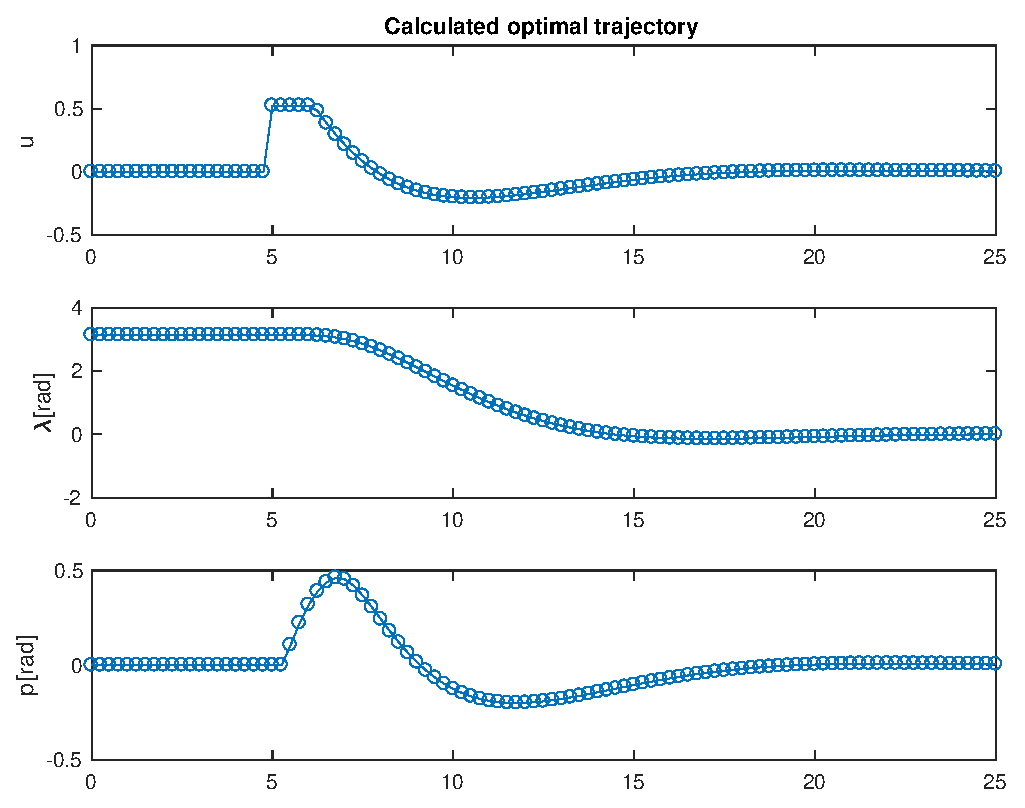
\includegraphics[scale=0.5]{data_10.2/All_states_q_10.eps}
    \caption{Calculated optimal trajectory showing input ($u$), travel ($\lambda$) and pitch ($p$) with $q = 10$.}
    \label{fig:10_2_q_10}
\end{figure}

As seen from the plots in the figures above, increased values of $q$ results in the input $u$ and pitch angle $p$ to maintain its maximum values for shorter periods, which also increases the time it takes for the helicopter to reach its target destination. However, for each value of $q$ both the input $u$ and the pitch angle $p$ reaches its maximum value, allowing for maximum possible speed. The value of $q$ determines how much the pitch angle should be penalized, relative to the state error, ($\lambda_i$ $-$ $\lambda_f$ )$^2$. When calculating an optimal trajectory with a large value of $q$, the pitch will be more penalized, while larger state errors will be allowed. This results in small variations in pitch angle. Likewise, a small value of $q$ will allow for more variation in pitch angle, while state errors will be more penalized. This can be seen from the plots in Figure \ref{fig:10_2_q_0.1}, \ref{fig:10_2_q_1} and \ref{fig:10_2_q_10}.\\

\begin{figure}[H]
\captionsetup{justification=centering}
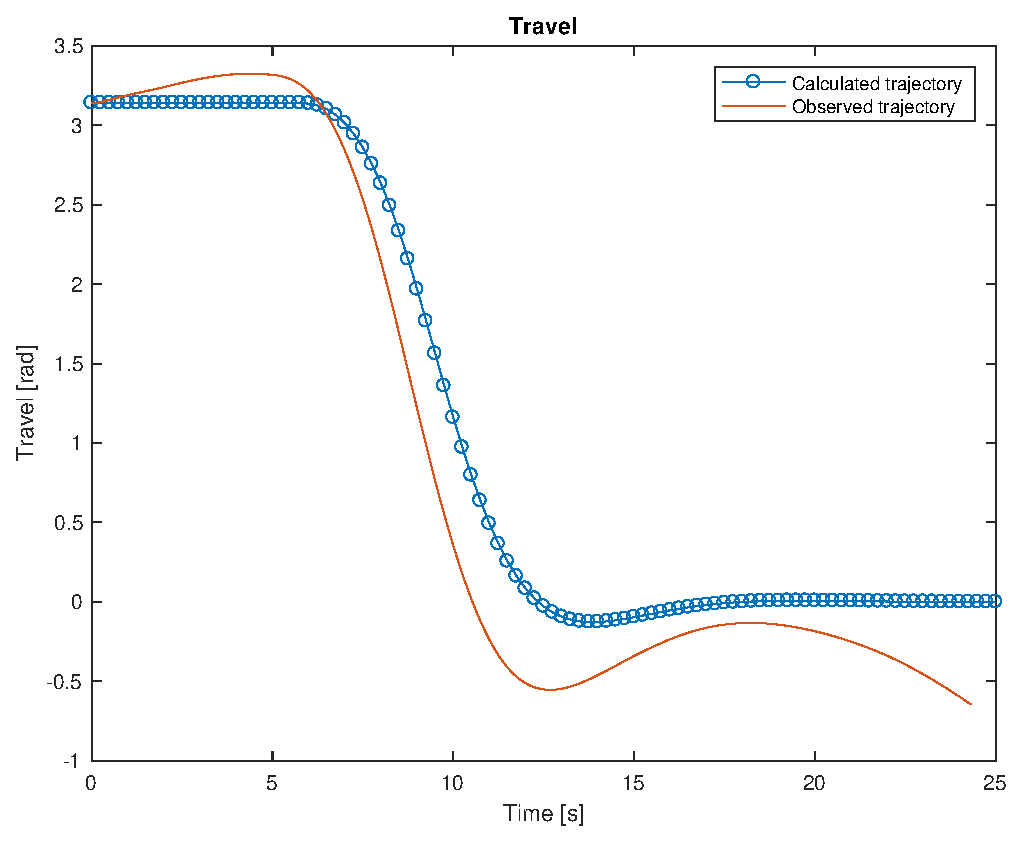
\includegraphics[scale=0.56]{data_10.2/Calculated_vs_Observed_Travel_q_1.eps} 
\centering
\caption{The calculated travel trajectory plotted against the observed travel trajectory with $q = 1$.}  \label{fig:travel_opt}
\end{figure}

\begin{figure}[H]
\captionsetup{justification=centering}
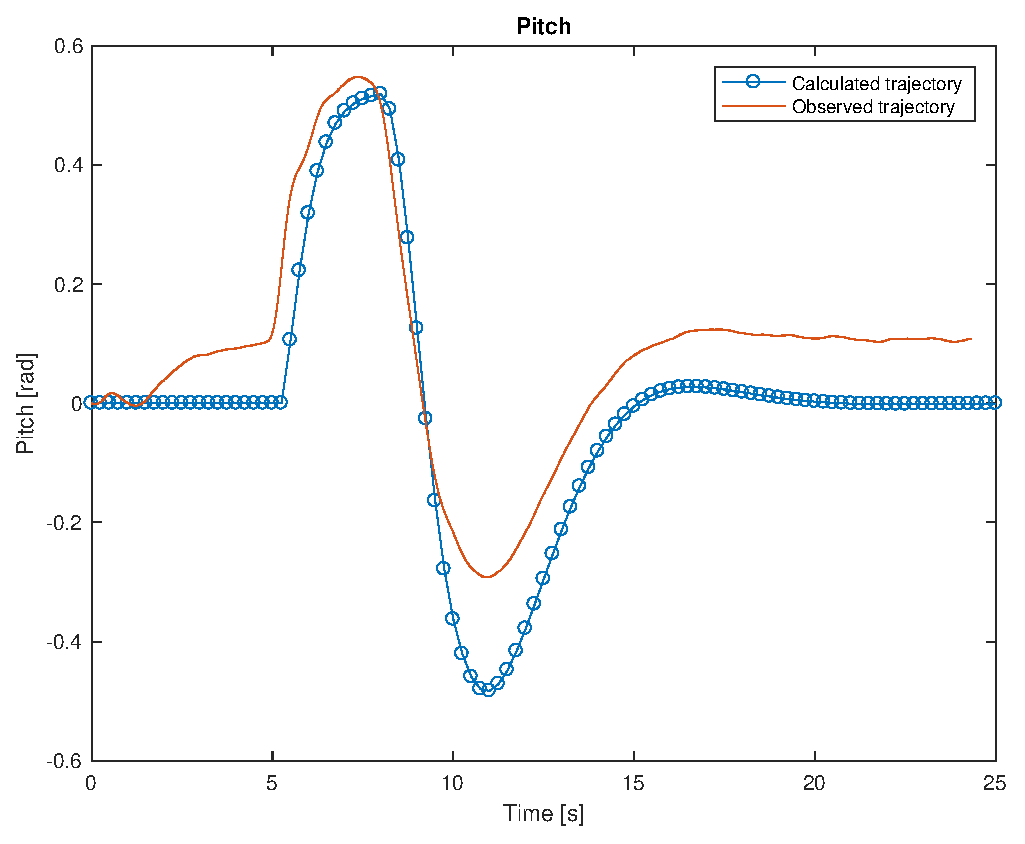
\includegraphics[scale=0.56]{data_10.2/Calculated_vs_Observed_Pitch_q_1.eps} 
\centering
\caption{The calculated pitch trajectory plotted against the observed pitch trajectory with $q = 1$.}
\label{fig:pitch_opt}
\end{figure}

Figure \ref{fig:travel_opt} and \ref{fig:pitch_opt} shows the calculated trajectory for travel and pitch plotted against the measured trajectory for travel and pitch, with $q = 1$. As seen from the plot in Figure \ref{fig:pitch_opt}, the helicopter started off with a small pitch angle, causing it to drift away from $\lambda = \pi$ as shown in Figure \ref{fig:travel_opt}. This means that even with a perfect model and no disturbances, the helicopter would not reach $\lambda = 0$, because the initial point differs from $\lambda = \pi$. However, a perfect system model and no disturbances on the system is unrealistic. A possible solution to this problem would be to implement feedback. This is not done in this section of the exercise, thus the helicopter does not end up in its desired state. Without feedback the helicopter will only follow what was scripted in the MATLAB-file, and with the mentioned imperfect model and disturbances, it is very hard to end up with a good result. 
